% Options for packages loaded elsewhere
\PassOptionsToPackage{unicode}{hyperref}
\PassOptionsToPackage{hyphens}{url}
%
\documentclass[
  ignorenonframetext,
]{beamer}
\usepackage{pgfpages}
\setbeamertemplate{caption}[numbered]
\setbeamertemplate{caption label separator}{: }
\setbeamercolor{caption name}{fg=normal text.fg}
\beamertemplatenavigationsymbolsempty
% Prevent slide breaks in the middle of a paragraph
\widowpenalties 1 10000
\raggedbottom
\setbeamertemplate{part page}{
  \centering
  \begin{beamercolorbox}[sep=16pt,center]{part title}
    \usebeamerfont{part title}\insertpart\par
  \end{beamercolorbox}
}
\setbeamertemplate{section page}{
  \centering
  \begin{beamercolorbox}[sep=12pt,center]{part title}
    \usebeamerfont{section title}\insertsection\par
  \end{beamercolorbox}
}
\setbeamertemplate{subsection page}{
  \centering
  \begin{beamercolorbox}[sep=8pt,center]{part title}
    \usebeamerfont{subsection title}\insertsubsection\par
  \end{beamercolorbox}
}
\AtBeginPart{
  \frame{\partpage}
}
\AtBeginSection{
  \ifbibliography
  \else
    \frame{\sectionpage}
  \fi
}
\AtBeginSubsection{
  \frame{\subsectionpage}
}
\usepackage{amsmath,amssymb}
\usepackage{lmodern}
\usepackage{iftex}
\ifPDFTeX
  \usepackage[T1]{fontenc}
  \usepackage[utf8]{inputenc}
  \usepackage{textcomp} % provide euro and other symbols
\else % if luatex or xetex
  \usepackage{unicode-math}
  \defaultfontfeatures{Scale=MatchLowercase}
  \defaultfontfeatures[\rmfamily]{Ligatures=TeX,Scale=1}
\fi
% Use upquote if available, for straight quotes in verbatim environments
\IfFileExists{upquote.sty}{\usepackage{upquote}}{}
\IfFileExists{microtype.sty}{% use microtype if available
  \usepackage[]{microtype}
  \UseMicrotypeSet[protrusion]{basicmath} % disable protrusion for tt fonts
}{}
\makeatletter
\@ifundefined{KOMAClassName}{% if non-KOMA class
  \IfFileExists{parskip.sty}{%
    \usepackage{parskip}
  }{% else
    \setlength{\parindent}{0pt}
    \setlength{\parskip}{6pt plus 2pt minus 1pt}}
}{% if KOMA class
  \KOMAoptions{parskip=half}}
\makeatother
\usepackage{xcolor}
\IfFileExists{xurl.sty}{\usepackage{xurl}}{} % add URL line breaks if available
\IfFileExists{bookmark.sty}{\usepackage{bookmark}}{\usepackage{hyperref}}
\hypersetup{
  pdftitle={Information choice and economic complexity},
  pdfauthor={Cameron Pfiffer},
  hidelinks,
  pdfcreator={LaTeX via pandoc}}
\urlstyle{same} % disable monospaced font for URLs
\newif\ifbibliography
\setlength{\emergencystretch}{3em} % prevent overfull lines
\providecommand{\tightlist}{%
  \setlength{\itemsep}{0pt}\setlength{\parskip}{0pt}}
\setcounter{secnumdepth}{-\maxdimen} % remove section numbering
\usepackage{/home/cameron/Dropbox/Presentations/cbeamer/cstyle}
\usepackage{booktabs}
\usepackage{graphicx}
\usepackage[labelformat=empty]{caption}
\usepackage{dcolumn}
\usepackage{anyfontsize}
\usepackage{adjustbox}
\usepackage[T1]{fontenc}
\usepackage{relsize}
\usepackage{bm}
\usepackage{physics}
\usepackage{booktabs}
\usepackage{longtable}
\usepackage{array}
\usepackage{multirow}
\usepackage{wrapfig}
\usepackage{float}
\usepackage{colortbl}
\usepackage{pdflscape}
\usepackage{tabu}
\usepackage{threeparttable}
\usepackage{threeparttablex}
\usepackage[normalem]{ulem}
\usepackage{makecell}
\usepackage{xcolor}
\usepackage{hhline}
\usepackage{adjustbox}
\usepackage{soul}
\ifLuaTeX
  \usepackage{selnolig}  % disable illegal ligatures
\fi

\title{Information choice and economic complexity}
\author{Cameron Pfiffer}
\date{October 1st, 2021}
\institute{University of Oregon}

\begin{document}
\frame{\titlepage}

\hypertarget{research-question}{%
\section{Research question}\label{research-question}}

\begin{frame}{Research question}
\protect\hypertarget{research-question-1}{}
How should you choose what information to analyze when the economy is
ex-ante complicated?

Alternatively, how much information is it \blue{rational to ignore}?
\end{frame}

\begin{frame}{Information choice}
\protect\hypertarget{information-choice}{}
\red{Information choice} is the study of how investors choose what
things they wish to know about.

In asset pricing, we like to think about how information choice impacts
things like

\begin{itemize}
\tightlist
\item
  Expected returns
\item
  Risk premia
\item
  Welfare (?)
\end{itemize}

I use ``information choice'' and ``attention'' synonymously.
\end{frame}

\begin{frame}{My hypothesis}
\protect\hypertarget{my-hypothesis}{}
I am trying to find out whether ``complex'' economies cause the basic
findings of information choice models to fall apart.

Common findings:

\begin{itemize}
\tightlist
\item
  When a ``common component'' of payoffs or returns becomes more
  volatile, more attention goes to the common component. Common
  component here might be the business cycle or market returns.
\item
  Increased attention reduces excess volatility, while decreased
  attention increases excess volatility.
\item
  Prices are informative about payoffs because prices are a function of
  investor attention.
\end{itemize}
\end{frame}

\begin{frame}{My hypothesis}
\protect\hypertarget{my-hypothesis-1}{}
What I think might happen:

\begin{itemize}
\tightlist
\item
  Investors allocate attention in a way that can systematically mislead
  them about the state of the economy.
\item
  Attention allocation can increase or decrease excess
  volatility/returns in a biased way.
\item
  Prices may be \red{very informative} or \blue{not informative at all},
  since investors with different information can interperet prices
  radically differently.
\end{itemize}

In short -- the
\textbf{findings of information choice models might not be as clear in complex economies}.
\end{frame}

\begin{frame}{Complexity}
\protect\hypertarget{complexity}{}
\begin{center}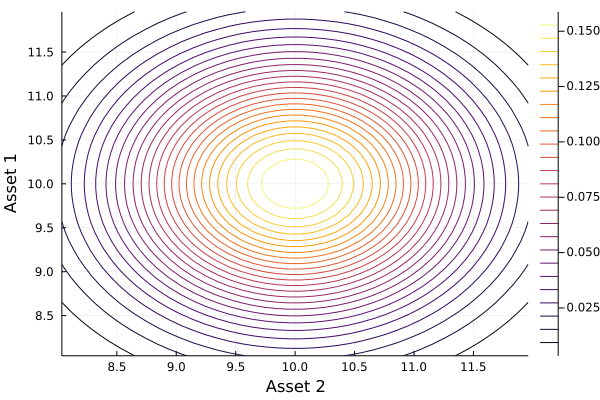
\includegraphics[width=0.9\paperheight]{complexity_files/figure-beamer/unnamed-chunk-2-1} \end{center}

Traditional models of information choice use unimodal joint densities
with good properties. The above is the case used in Kacperczyk et
al.~(2016).
\end{frame}

\end{document}
